\begin{columns}
  \begin{column}{0.45\textwidth}
    \begin{center}
      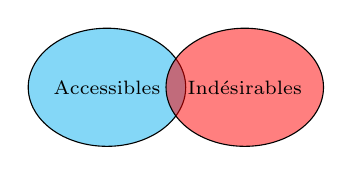
\begin{tikzpicture}
        \draw[fill=ProcessBlue, fill opacity=0.5] (0,0) ellipse (1 and 0.75);
        \node (r*i) at (0,0) {\scriptsize{Accessibles}};
        \draw[fill=Red, fill opacity=0.5] (1.75,0) ellipse (1 and 0.75);
        \node (bad) at (1.75,0) {\scriptsize{Indésirables}};
      \end{tikzpicture}\\
      Il existe une configuration\\ indésirable accessible
    \end{center}
  \end{column}
  \begin{column}{0.45\textwidth}
    \begin{center}
      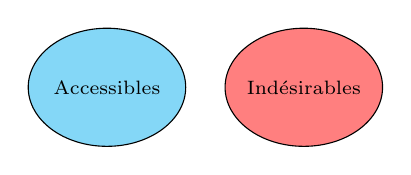
\begin{tikzpicture}
        \draw[fill=ProcessBlue, fill opacity=0.5] (0,0) ellipse (1 and 0.75);
        \node (r*i) at (0,0) {\scriptsize{Accessibles}};
        \draw[fill=Red, fill opacity=0.5] (2.5,0) ellipse (1 and 0.75);
        \node (bad) at (2.5,0) {\scriptsize{Indésirables}};
      \end{tikzpicture}\\
      Aucune configuration indésirable\\ n'est accessible
    \end{center}
  \end{column}
\end{columns}